\documentclass[a4paper,12pt]{article} % тип документа

% Поля страниц
\usepackage[left=2.5cm,right=2.5cm,
    top=2cm,bottom=2cm,bindingoffset=0cm]{geometry}
    
%Пакет дял таблиц   
\usepackage{multirow} 
    
%Отступ после заголовка    
\usepackage{indentfirst}


% Рисунки
\usepackage{floatrow,graphicx,calc}
\usepackage{wrapfig}

%%% Работа с картинками
\usepackage{graphicx}  % Для вставки рисунков
\graphicspath{{images/}{images2/}}  % папки с картинками
\setlength\fboxsep{3pt} % Отступ рамки \fbox{} от рисунка
\setlength\fboxrule{1pt} % Толщина линий рамки \fbox{}
\usepackage{wrapfig} % Обтекание рисунков и таблиц текстом

% Создаёем новый разделитель
\DeclareFloatSeparators{mysep}{\hspace{1cm}}

% Ссылки?
\usepackage{hyperref}
\usepackage[rgb]{xcolor}
\hypersetup{				% Гиперссылки
    colorlinks=true,       	% false: ссылки в рамках
	urlcolor=blue          % на URL
}


%  Русский язык
\usepackage[T2A]{fontenc}			% кодировка
\usepackage[utf8]{inputenc}			% кодировка исходного текста
\usepackage[english,russian]{babel}	% локализация и переносы




% Математика
\usepackage{amsmath,amsfonts,amssymb,amsthm,mathtools}

%%% Дополнительная работа с математикой
\usepackage{amsmath,amsfonts,amssymb,amsthm,mathtools} % AMS
\usepackage{icomma} % "Умная" запятая: $0,2$ --- число, $0, 2$ --- перечисление


% Что-то 
\usepackage{wasysym}


\begin{document}
\begin{center}
	\footnotesize{ФЕДЕРАЛЬНОЕ ГОСУДАРСТВЕННОЕ АВТОНОМНОЕ ОБРАЗОВАТЕЛЬНОЕ 			УЧРЕЖДЕНИЕ ВЫСШЕГО ОБРАЗОВАНИЯ}\\
	\footnotesize{МОСКОВСКИЙ ФИЗИКО-ТЕХНИЧЕСКИЙ ИНСТИТУТ\\(НАЦИОНАЛЬНЫЙ 			ИССЛЕДОВАТЕЛЬСКИЙ УНИВЕРСИТЕТ)}\\
	\footnotesize{ФАКУЛЬТЕТ ОБЩЕЙ И ПРИКЛАДНОЙ ФИЗИКИ\\}
	\hfill \break
	\hfill \break
	\hfill \break
	\hfill \break
\end{center}


\begin{figure*}[h]
    \centering
    \includegraphics*[width=10cm,height=7cm,keepaspectratio]{mipt_eng_text_png.png}
    \label{fig:my_label}
\end{figure*}


\begin{center}   
    \hfill \break
	\hfill \break
	\hfill \break
	\large{Лабораторная работа № 4.3.1\\ \hfill \break\Large{Изучение дифракции света}}\\
	\hfill \break
	\hfill \break
	\hfill \break
	\hfill \break
	\begin{flushright}
		Баранов Даниил\\
		Группа Б02-103
	\end{flushright}
	\hfill \break
	\hfill \break
	\hfill \break
\end{center}
\hfill \break
\hfill \break
\hfill \break
\hfill \break
\begin{center}
	Долгопрудный, 2023 г.
\end{center}
\thispagestyle{empty}

\newpage

\textbf{Цель:} исследовать явления дифракции Френеля и Фраунгофера на щели, изучить влияние дифракции на разрешающую способность оптических инструментов.


\textbf{Оборудование:} оптическая скамья, ртутная лампа, мо- нохроматор, щели с регулируемой шириной, рамка с вертикальной нитью, двойная щель, микроскоп на поперечных салазках с микро- метрическим винтом, зрительная труба.

\section{Теоретическая справка}
\subsection{Дифракция Френеля на щели}

Схема установки для наблюдения дифракции Френеля на щели представлена на рис. \ref{labA}. Световые лучи освещают щель $ S_2 $ и испытывают на ней дифракцию. Дифракционная картина рассматривается с помощью микроскопа М, сфокусированного на некоторую плоскость наблюдения П.

\begin{figure}[H]
	\centering
	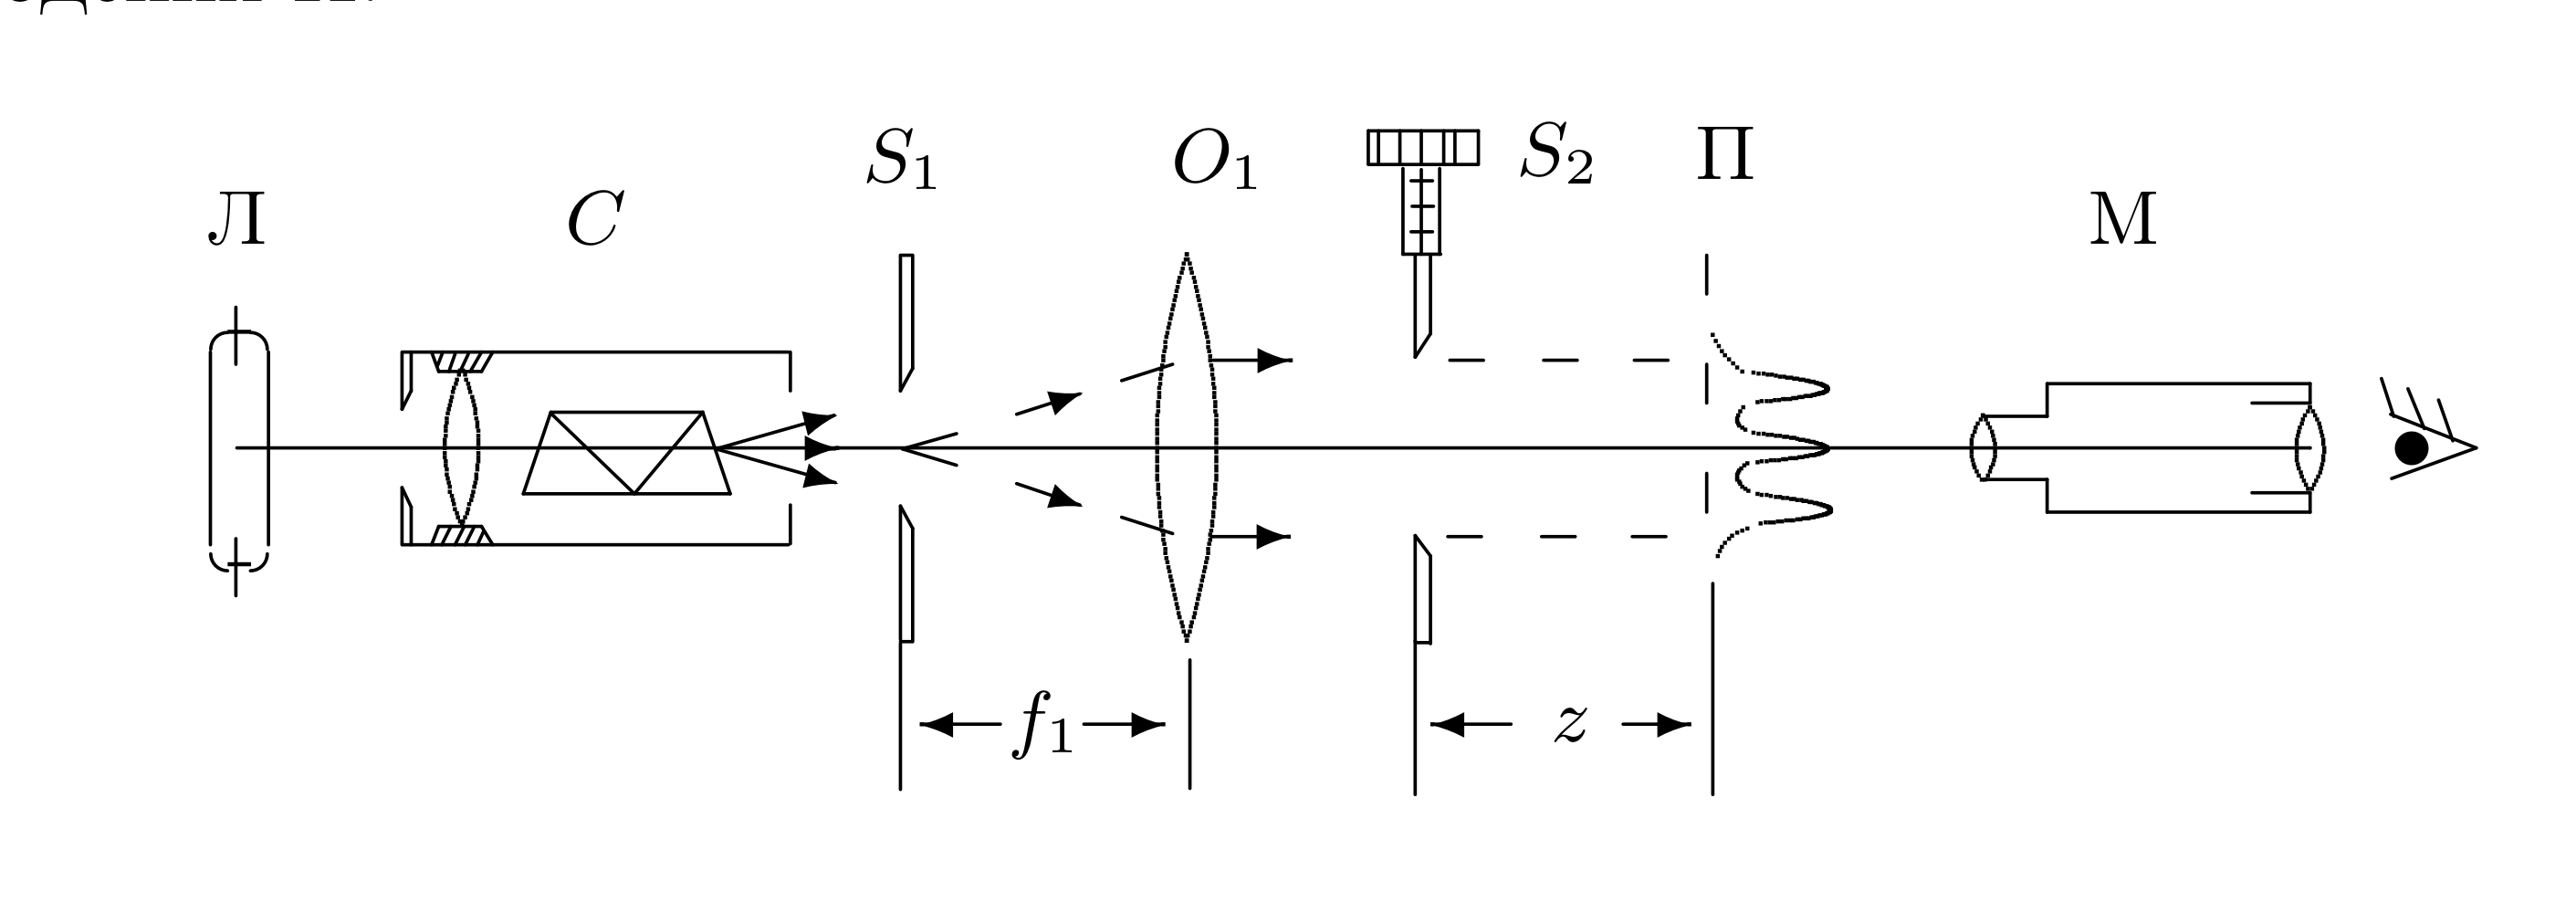
\includegraphics[scale=0.15]{4.3.1/alab.jpeg}
	\caption{Схема установки для наблюдения дифракции Френеля}
	\label{labA}
\end{figure}

Щель $ S_2 $ освещается параллельным пучком монохроматического света с помощью коллиматора, образованного объективом $ O_1 $, и щелью $S_1$, находящейся в его фокусе. На щель $ S_1 $ сфокусировано изображение спектральной линии, выделенной из спектра ртутной лампы Л при помощи простого монохроматора C, в котором используется призма прямого зрения. Распределение интенсивности света в плоскости наблюдения П проще всего рассчитывать с помощью зон Френеля (для щели их иногда называют зонами Шустера). При освещении щели $ S_2 $ параллельным пучком лучей (плоская волна) зоны Френеля представляют собой полоски, параллельные краям щели (рис. \ref{zone}). Результирующая амплитуда в точке наблюдения определяется суперпозицией колебаний от тех зон Френеля, которые не перекрыты створками щели. Графическое определение результирующей амплитуды производится с помощью векторной диаграммы --- спирали Корню. Суммарная ширина $ n $ зон Френеля (Шустера) определяется соотношением:

\begin{equation}\label{xin}
\xi_n = \sqrt{zn\lambda}
\end{equation}
где $ z $ --- расстояние от щели до плоскости наблюдения (рис. \ref{labA}), а $ \lambda $ --- длина волны.

\begin{figure}[H]
	\begin{center}
		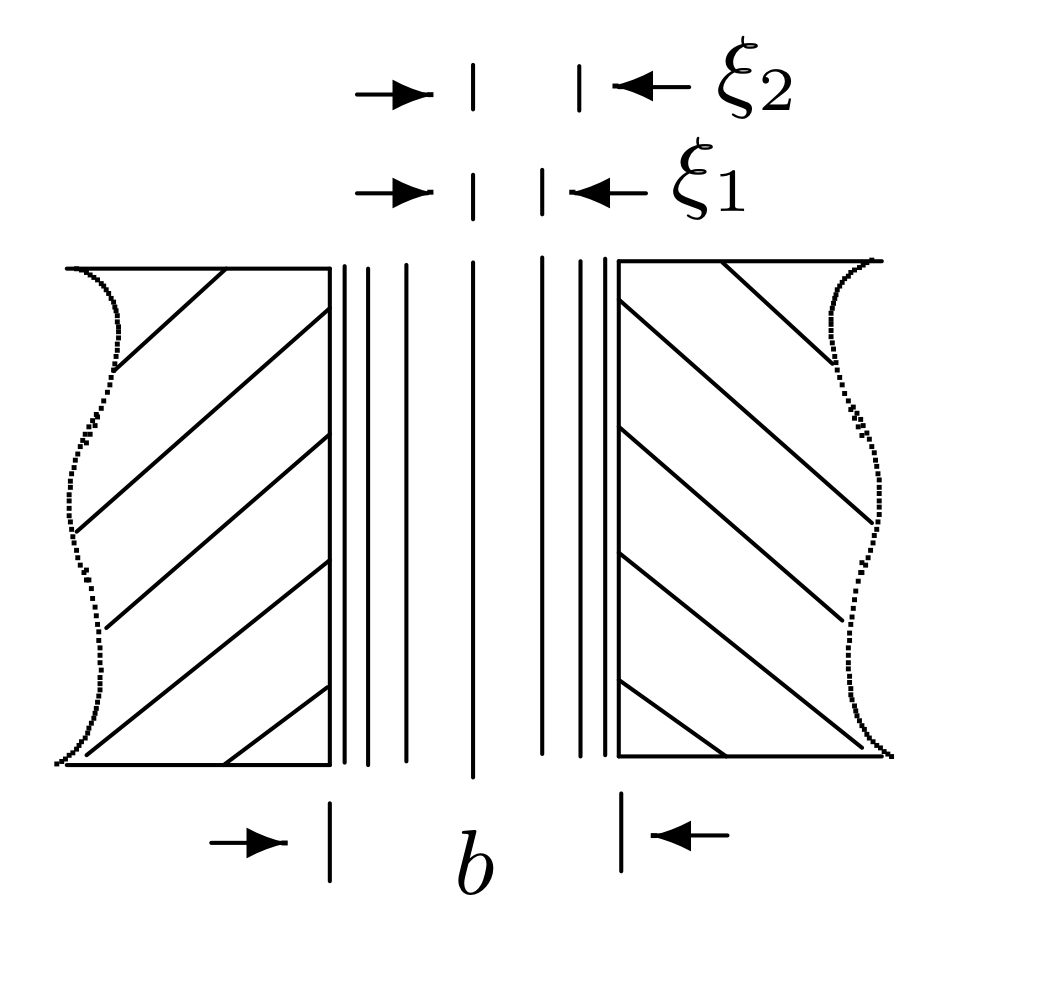
\includegraphics[scale=0.15]{4.3.1/zone.jpeg}
	\end{center}
	\caption{Зоны Френеля}
	\label{zone}
\end{figure}

Вид наблюдаемой дифракционной картины
на щели шириной $ b $ определяется волновым параметром $ p $ или числом Френеля $ C $ (число открытых полных зон):


\begin{equation}\label{}
p = \dfrac{\sqrt{z \lambda}}{b}, \qquad C = \dfrac{1}{p^2}
\end{equation}




\subsection{Дифракция Фраунгофера на одной щели}

На значительном удалении от щели, когда выполнено условие $ C \ll 1 $
(то есть ширина щели становится значительно меньше ширины первой
зоны Френеля, $ b \ll \sqrt{\lambda z} $), изображение щели размывается и возникает
дифракционная картина, называемая дифракцией Фраунгофера.

Дифракцию Френеля и Фраунгофера можно наблюдать на одной
и той же установке (рис. \ref{labA}). Однако при обычных размерах установки дифракция Фраунгофера возникает только при очень узких щелях.

\begin{figure}[H]
	\centering
	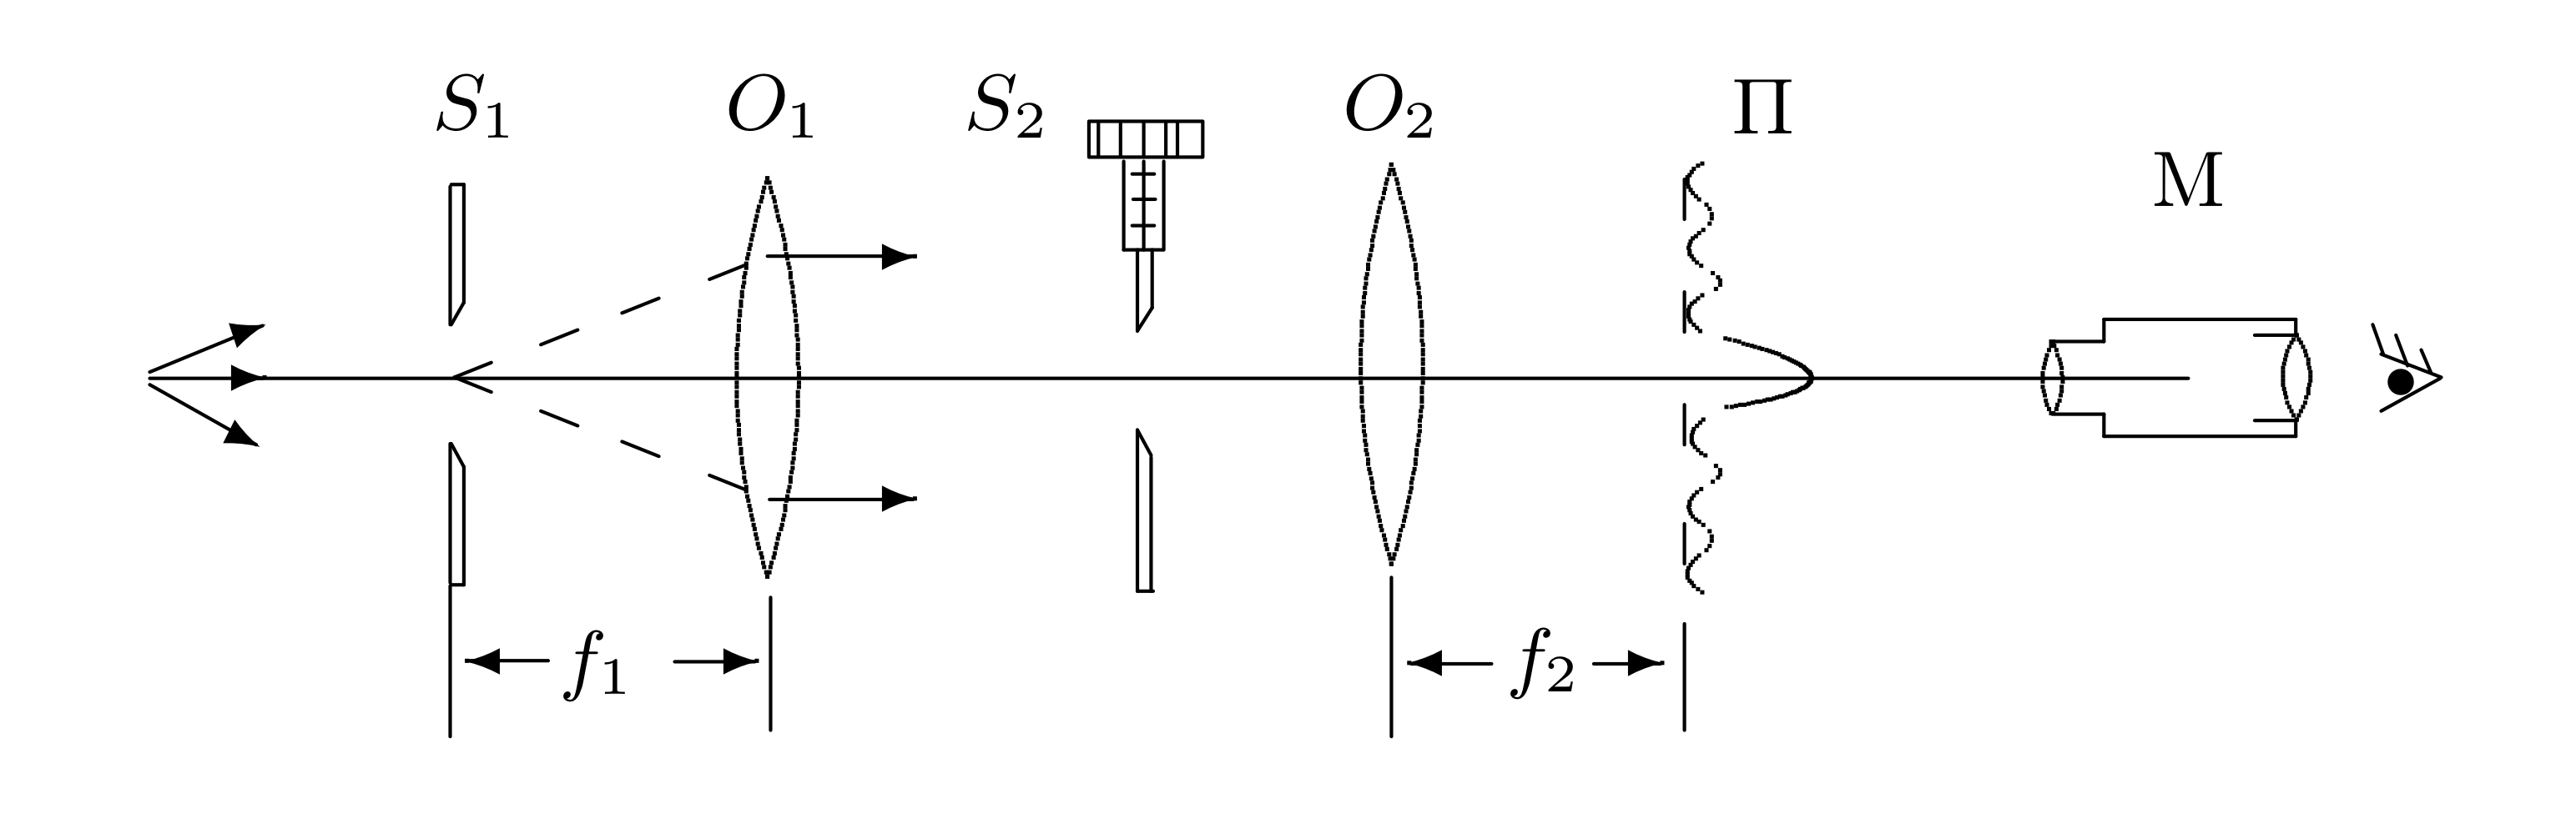
\includegraphics[scale=0.15]{4.3.1/blab.jpeg}
	\caption{Схема установки для наблюдения дифракции Фраунгофера на щели}
	\label{labB}
\end{figure}

Например, при $ z \approx  20-40 $  см и $  \lambda \approx 5 \cdot 10^{-5}  $   см получаем $  b \ll 0,3 $ мм. Поскольку работать с такими тонкими щелями неудобно, для наблюдения дифракции Фраунгофера к схеме, изображённой на рис. \ref{labA}, добавляется объектив $ O_2  $ (рис. \ref{labB}).

Дифракционная картина наблюдается здесь в фокальной плоскости
объектива $ O_2 $. Каждому значению угла $ \theta $ соответствует в этой плоскости точка, отстоящая от оптической оси на расстоянии

\begin{equation}\label{x}
x = f_2 \tg \theta \approx f_2 \theta
\end{equation}


плоскости наблюдается неискаженная дифракционная картина Фраунгофера. Эта картина соответствует бесконечно удалённой плоскости
наблюдения.

В центре поля зрения наблюдается дифракционный максимум (светлая полоса). При малых углах $ \theta $ положение минимумов (тёмных полос)
определяется, соотношением

\begin{equation}\label{theta_m}
\theta_m = m \dfrac{\lambda}{b}
\end{equation}

Расстояние $ x_m $ от тёмной полосы до оптической оси объектива $ O_2 $ пропорционально фокусному расстоянию $ f_2 $. Из \eqref{x} и \eqref{theta_m} следует 

\begin{equation}\label{xm}
x_m = m \dfrac{\lambda}{b} f_2
\end{equation}

Видно, что при малых углах минимумы эквидистантны, а расстояния $ \delta x $ между минимумами обратно пропорциональны ширине $ b $ щели $ S_2 $.



\subsection{Дифракция Фраунгофера на двух щелях}

Для наблюдения дифракции Фраунгофера на двух щелях в установке (рис. \ref{labB}) следует заменить щель $ S_2 $ экраном Э с двумя щелями
(рис. \ref{labC}). При этом для оценки влияния ширины входной щели на чёткость дифракционной картины вместо входной щели $ S_1 $ следует поставить щель с микрометрическим винтом. Два дифракционных изображения входной щели, одно из которых образовано лучами, прошедшими через левую, а другое --- через правую щели, накладываются друг на друга.

\begin{figure}[H]
	\centering
	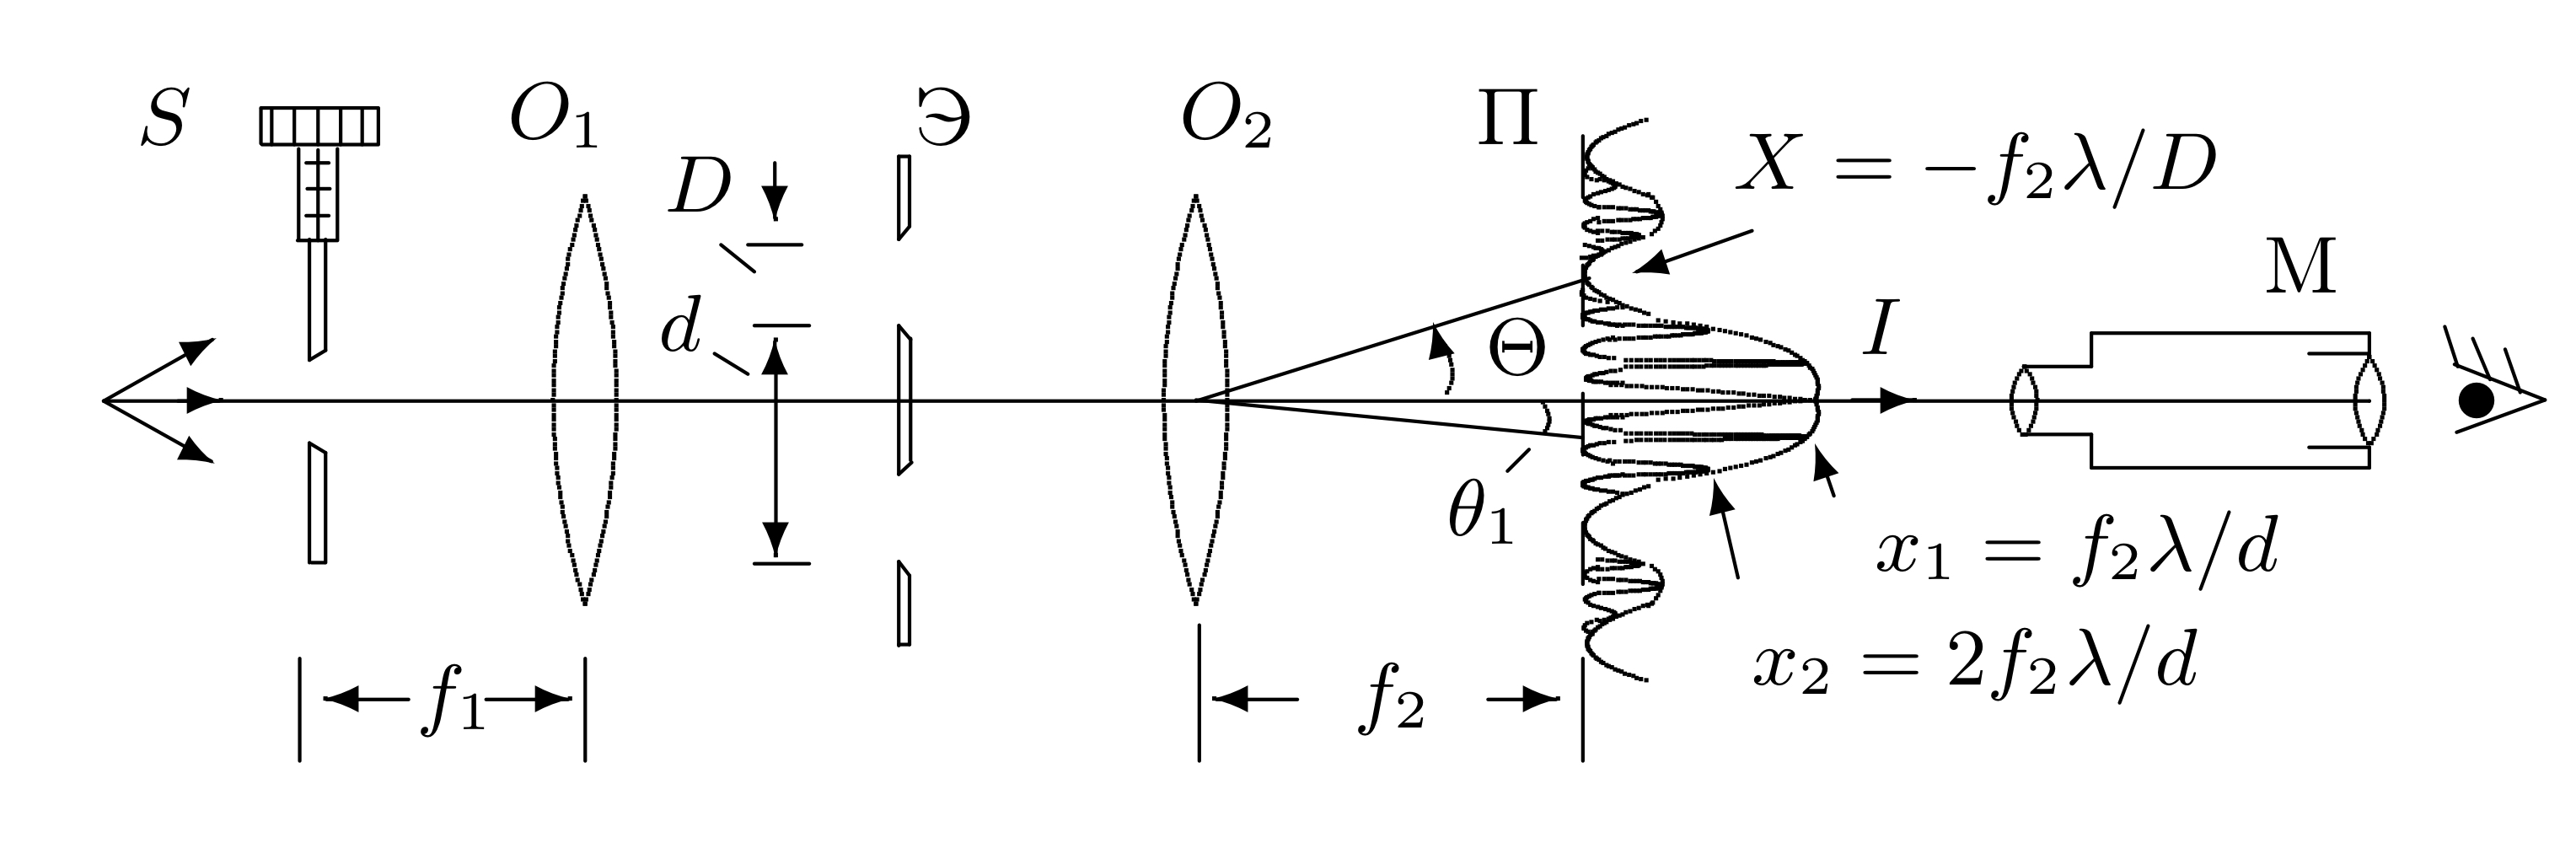
\includegraphics[scale=0.15]{4.3.1/clab.jpeg}
	\caption{Схема установки для наблюдения дифракции Фраунгофера на двух щелях}
	\label{labC}
\end{figure}

Если входная щель достаточно узка, то дифракционная картина
в плоскости П (рис. \ref{labC}) подобна той, что получалась при дифракции
на одной щели (рис. \ref{labB}), однако теперь вся картина испещрена рядом
дополнительных узких полос.
Угловая координата $ \theta_m $ интерференционного максимума $ m $-го порядка определяется соотношением

\begin{equation}\label{}
\theta_m = m \dfrac{\lambda}{b}
\end{equation}

где $ d $ --- расстояние между щелями. Линейное расстояние $ \delta x $ между соседними интерференционными полосами в плоскости П равно, поэтому

\begin{equation}\label{dx}
\delta x = f_2 \dfrac{\lambda}{d}
\end{equation}

На рис. \ref{labC} показано распределение интенсивности в фокальной плоскости объектива $ O_2 $. Штриховой линией (в увеличенном масштабе)
изображено распределение интенсивности при дифракции света на одиночной щели. Нетрудно оценить число n интерференционных полос,
укладывающихся в области центрального дифракционного максимума.
Согласно \eqref{xm} полная ширина главного максимума равна $ 2 f_2 \lambda /b $, где $ b $ ширина щели, отсюда

\begin{equation}\label{n}
n = \dfrac{2f_2 \lambda}{b} \dfrac{1}{\delta x} = \dfrac{2d}{b}
\end{equation}

При дифракции света на двух щелях чёткая система интерференционных полос наблюдается только при достаточно узкой ширине входной щели $ S $, которую можно рассматривать как протяжённый источник света размером $ b $. Для наблюдения интерференции необходимо, чтобы расстояние $ d $между щелями не превышало радиуса когерентности

\begin{equation}\label{}
d \ll \dfrac{\lambda}{b} f_1
\end{equation}

Здесь $ b $ --- ширина входной щели $ S $ и, следовательно, $  b/f_1 $ --- её угловая ширина. Таким образом, по размытию интерференционной картины можно оценить размер источника. Этот метод используется в звёздном интерферометре при измерении угловых размеров звёзд.

\subsection{Влияние дифракции на разрешающую способность оптического инструмента}

Установка, представленная на рис. \ref{labB}, позволяет исследовать влияние дифракции на разрешающую способность оптических инструментов.

Как уже было выяснено, линзы $O_1$ и $ O_2$ в отсутствие щели $S_2$ создают в плоскости П изображение щели $S_1$, и это изображение рассматривается в микроскоп М. Таким образом, нашу установку можно рассматривать как оптический инструмент, предназначенный для получения изображения предмета. При этом коллиматор (щель $S_1$ и объектив $O_1$) является моделью далёкого предмета, а объектив $O_2$ и микроскоп М составляют зрительную трубу, наведённую на этот предмет.
Щель $S_2$, установленная непосредственно перед объективом $O_2$, позволяет изменять эффективный размер объектива и, следовательно, разрешающую способность оптической системы.

\begin{figure}[H]
	\centering
	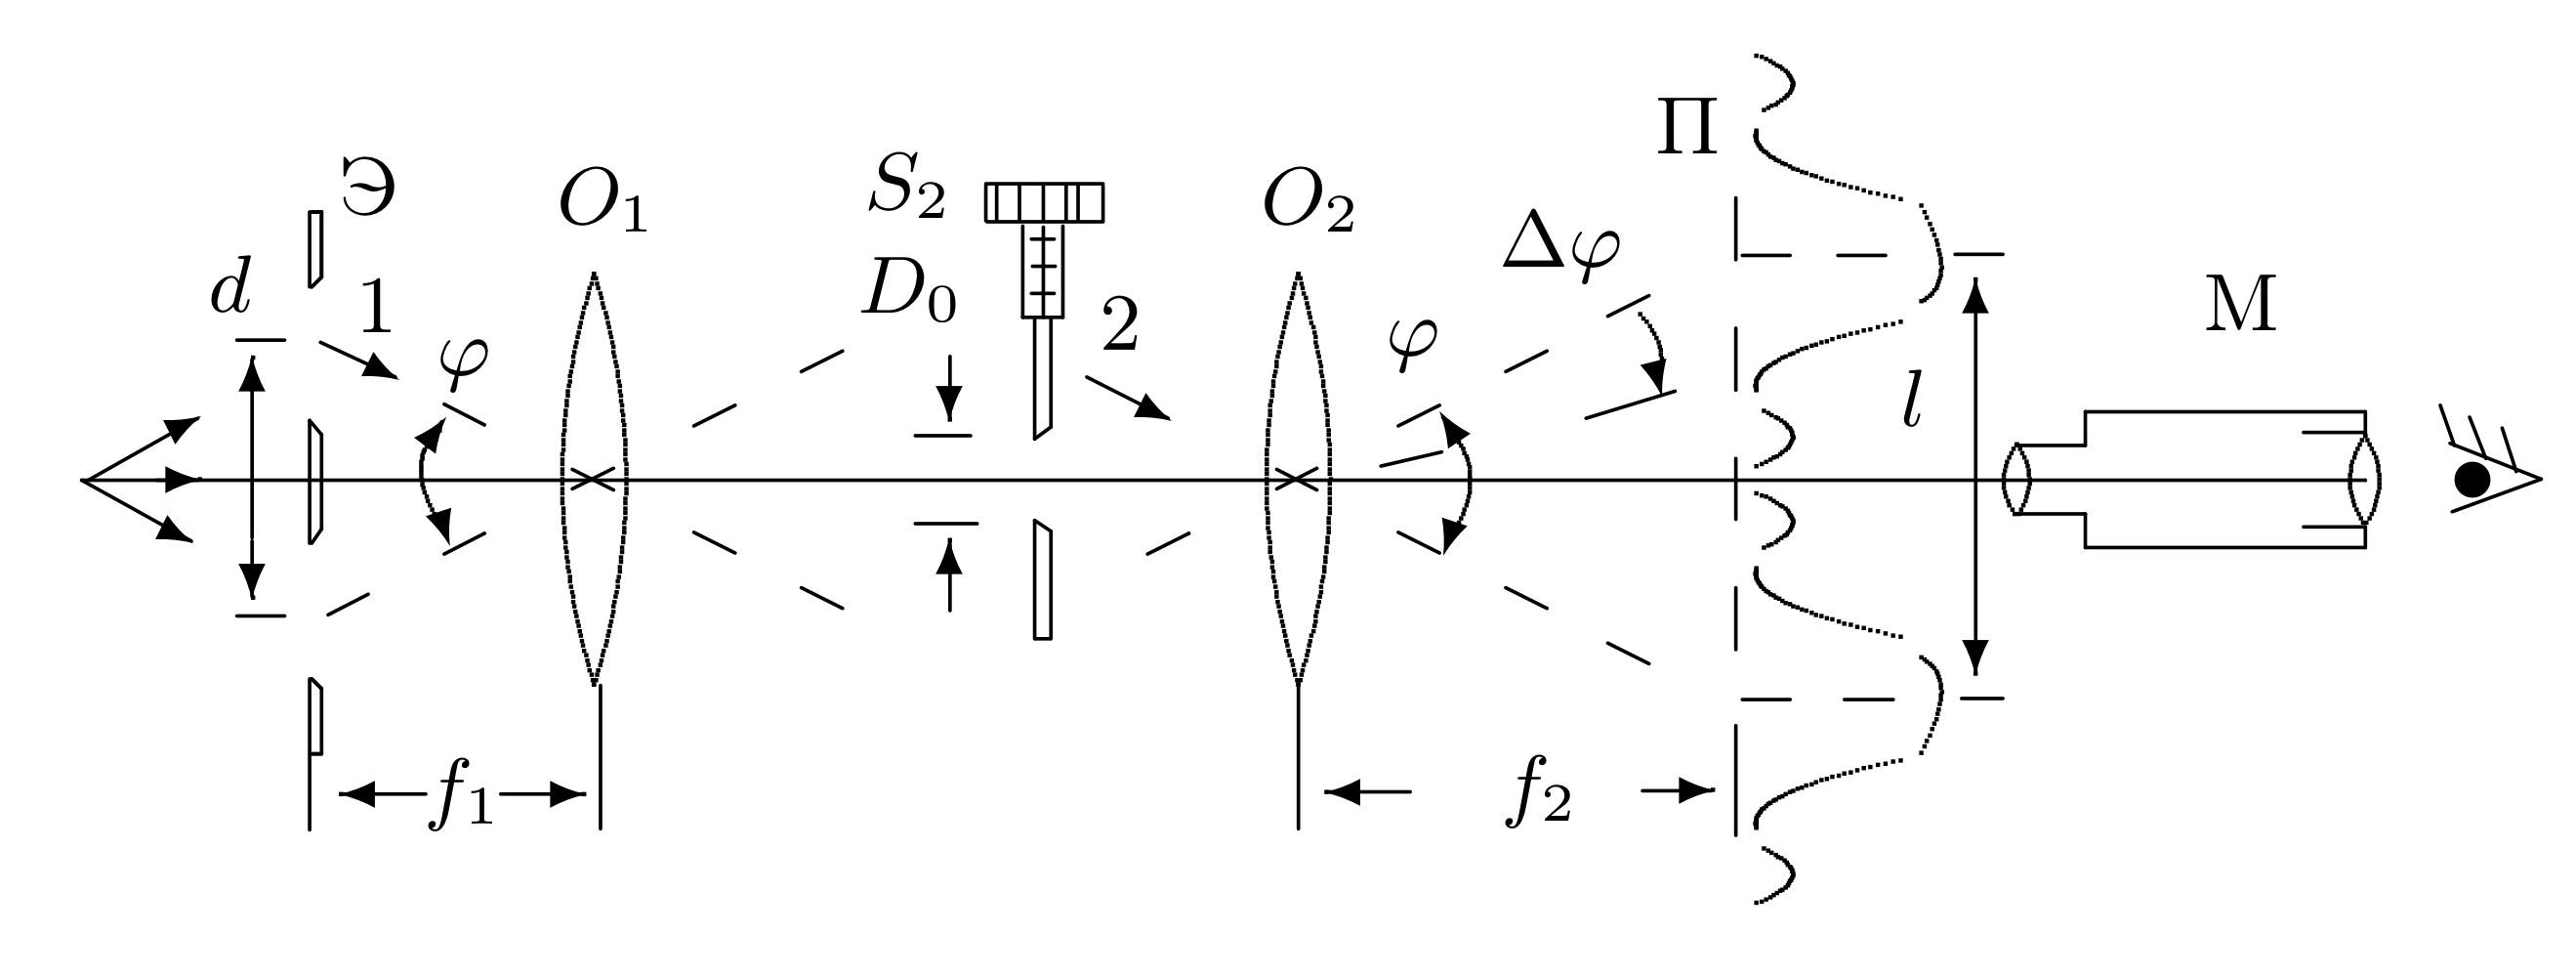
\includegraphics[scale=0.15]{4.3.1/dlab.jpeg}
	\caption{Схема установки для исследования разрешающей
		способности оптического инструмента}
	\label{labG}
\end{figure}

Поместим вместо щели $S_1$ экран Э с двумя узкими щелями, расстояние между которыми равно $d$ (рис. \ref{labG}). Тогда расстояние $l$ между изображениями щелей в плоскости П равно
\begin{equation}
l = \varphi f_2 = d \dfrac{f_2}{f_1},
\end{equation}
а ширина каждого изображения
\begin{equation}
\delta x \approx \dfrac{\lambda}{b} f_2
\end{equation}
определяется дифракцией света на щели $S_2$. Когда полуширина дифракционного изображения превышает расстояние между изображениями, то по виду дифракционной картины трудно определить, представляет собой источник двойную или одиночную щель.

Условия, при которых ещё можно различить, имеем мы дело с одной или двумя щелями, для разных наблюдателей различны. Для того чтобы исключить связанный с этим произвол, пользуются обычно критерием Рэлея, который приблизительно соответствует возможностям визуального наблюдения: изображения считаются различимыми, когда максимум одного дифракционного пятна совпадает с минимумом другого, а в условиях нашей задачи --- когда полуширина дифракционного изображения $\delta x$ совпадает с расстоянием $l$ между изображениями отдельных щелей:
\begin{equation}
\delta x \sim l \to \dfrac{\lambda}{b} \sim \dfrac{d}{f_1}.
\end{equation}

\section{Измерения и обработка результатов}

\subsection{Дифракция Френеля на щели}

Измерим первоначальную длину щели: $ b = 0,27 \pm 0,01$ мм. Будем приближать микроскоп к щели, по мере этого снимем зависимость координаты микроскопа от числа $ n  $ тёмных полос по формуле $ z_n = x_n - x_0 $, где $ x_0 = 611 $ мм --- положение нуля. Результаты занесём в таб. \ref{table1}. В таблицу также занесём результат вычисления величины $ 2\xi_n $ по формуле \eqref{xin}. При этом длина волны зелёного света $ \lambda = 5461 \cdot 10^{-10} $ м. 
\begin{equation}
\xi_n = \sqrt{zn\lambda}.
\end{equation}

\floatsetup[table]{capposition=top}

\begin{table}[H]
	\caption{Зависимость координаты микроскопа от числа $ n $ тёмных полос}
	\label{table1}	
	\begin{center}
		\begin{tabular}{|c|c|c|c|c|}
			\hline
			$ x_n $, мм  & $ z_n $, мм & $ n $& $ 2\xi_n $, мм& $ \sigma_{2\xi_n} $, мм\\
			\hline
			591 &	20	&	1   & 0,21  & 0,01
			\\ \hline
			596	&	15	&	2   & 0,26  & 0,01
			\\ \hline
			600	&	11	&	3   & 0,27  & 0,01
			\\ \hline
			602	& 	9	&	4   & 0,28  & 0,01
			\\ \hline
			604	&	7	&	5   & 0,28  & 0,01	\\
			\hline
            605	&	6	&	6   & 0,28  & 0,01	\\
			\hline
		\end{tabular}
	\end{center}

\end{table}

Полученные данные можно сравнить с установленной шириной щели ($ b = 0,27 \pm 0,01$).

\subsection{Дифракция Фраунгофера на одной щели}

Величина щели по винту равна $ b = (0,27\pm0,01)$ мм. Фокусное расстояние линзы $ f_2 = 16$ см.

Измерим с помощью винта поперечного перемещения микроскопа координаты $ x_m $ нескольких дифракционных минимумов.
Результаты занесём в таб \ref{tab2} и построим график зависимости минимумов от их номеров. 

\begin{table}[H]
	\caption{Зависимость минимумов от их номера $ m $}
	\begin{center}
		\begin{tabular}{|c|c|c|c|c|c|c|c|c|c|} \hline
			$m$ & -4 & -3 & -2 & -1 & 0 & 1 & 2 & 3 & 4\\ \hline
			$ x_m $, мм  & 0,40 & 0,60 & 0,87 & 1,12 & 1,40 & 1,68 & 1,90 & 2,14 & 2,40 \\ \hline
		\end{tabular}
	\end{center}
	\label{tab2}
\end{table}



\begin{figure}[H]
    \centering
    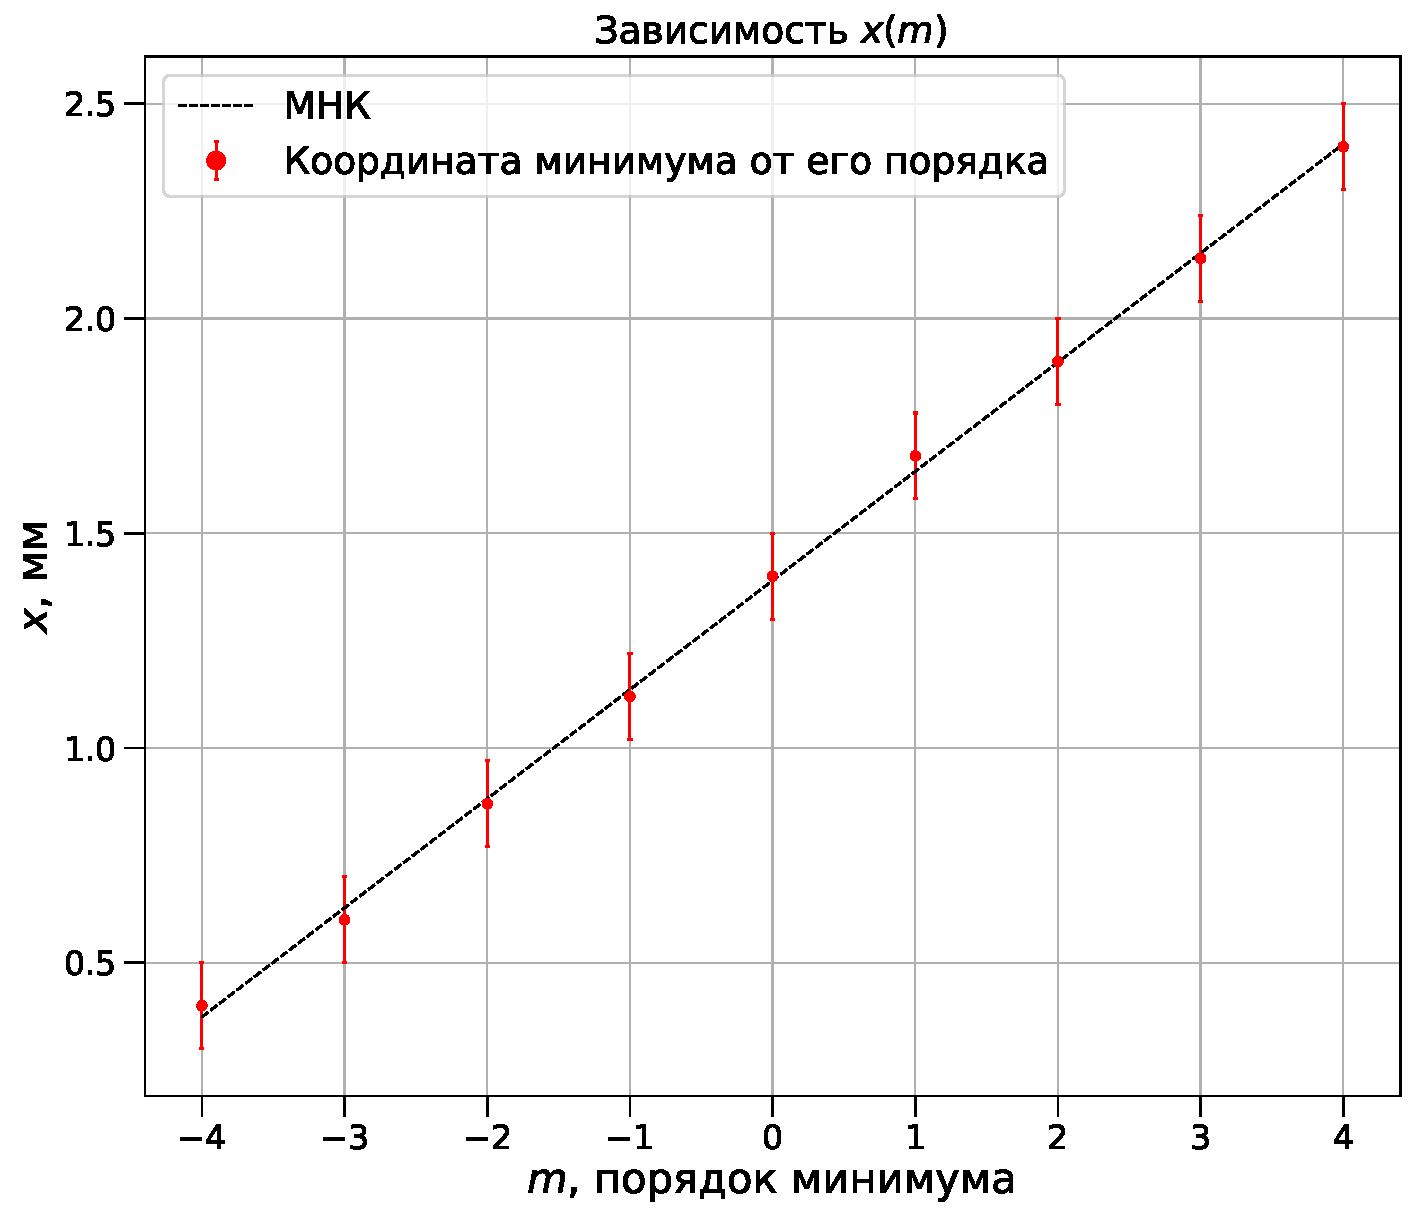
\includegraphics[scale=0.65]{4.3.1/x(m).pdf}
    \caption{График зависимости $x(m)$}
    \label{fig:my_label}
\end{figure}

Из графика получаем, что угол наклона $ K = 25,4 \pm 0,3 \cdot 10^{-2}  $ мм. Из формулы \eqref{xm} мы получаем, что 

\begin{equation}\label{qqq}
b =  \dfrac{\lambda}{K} f_2 =  3,36 \pm 0,04 \cdot 10^{-2} \; \text{мм}. 
\end{equation}

\subsection{Дифракция Фраунгофера на двух щелях}

Получим на экране дифракционную картину и проведём измерения и вычисления:

\begin{table}[H]
	\centering
	\caption{Измерения}
	\begin{tabular}{|c|c|c|c|c|} \hline
		$N$ &	$x$, мкм &	$\delta x$, мкм & $d$, мм & $b$, мкм \\
		\hline
		13	&	82 $\pm$ 1  & 6,3 $\pm$ 0,1 &	13,8 $\pm$ 0,5 &	49 $\pm$ 2 \\ \hline
	\end{tabular}   
\end{table}

Здесь $N$ --- число полос внутри главного максимума, $x$ --- ширина главного максимума, $\delta x = x/n$ --- расстояние между соседними интерференционными полосами, $d = f_2 \lambda/\delta x$ --- расстояние между щелями, $b = 2d/n$ --- ширина щели.

Также при помощи микроскопа измерим параметры щелей $ d $ и $ b $ <<напрямую>>. Получаем
\[ d_\text{микр} = 15,8 \pm 0,1 \text{ мм} \]
\[ b_\text{микр} = 49 \pm 0,1 \text{ мкм} \]

\subsection{Влияние дифракции на разрешающую способность оптического инструмента}

Для проверки справедливости критерия Рэлея сравним измеренную ширину $b_0$ щели $S_2$, при которой изображение двух щелей сливается, но всё ещё различимо, с расчётом по формуле $\lambda f_1/d$.

\begin{table}[H]
	\centering
	\caption{Измерения}
	\begin{tabular}{|c|c|} \hline
		$b_0$, мкм &	$\lambda f_1/d$, мкм \\
		\hline
		64 &	49 \\ \hline
	\end{tabular}   
\end{table}


\end{document}
